\documentclass[aspectratio=169]{beamer}

\usetheme{Madrid}
\usecolortheme{default}
\usepackage[utf8]{inputenc}
\usepackage[T1]{fontenc}
\usepackage{booktabs}
\usepackage{graphicx}

\setbeamertemplate{navigation symbols}{}
\setbeamertemplate{footline}[frame number]

\title{MLPC 2026 Task 4: Case Study and Reflection}
\subtitle{Classification Results on Held-Out Domestic Sound Events}
\author{Team A-C (Qualitative) \\ Julian Schmidt, Paul Breburda}
\date{May 2026}

\begin{document}

\begin{frame}
  \titlepage
\end{frame}

%% Slide 1: Final classifier context
\begin{frame}{Final Model and Evaluation Setup}
  \begin{columns}[T]
    \begin{column}{0.52\textwidth}
      \textbf{Setup:}
      \begin{itemize}
        \item Collector-disjoint train/validation/test split
        \item Majority-vote segment labels from $[T,C,A]$ annotations
        \item Macro average precision used for model selection
        \item Final model: validation-selected MLP probability ensemble
      \end{itemize}
      \vspace{0.4em}
      \textbf{Why macro AP:}
      \begin{itemize}
        \item Threshold-free for multi-label sigmoid outputs
        \item Gives rare classes equal weight
        \item Avoids hiding \texttt{light\_switch}/\texttt{bell} errors behind common classes
      \end{itemize}
    \end{column}
    \begin{column}{0.42\textwidth}
      \centering
      \small
      \begin{tabular}{lcc}
        \toprule
        Model & Macro AP & Micro AP \\
        \midrule
        Prior & 0.064 & 0.121 \\
        Logistic & 0.529 & 0.664 \\
        MLP ensemble & \textbf{0.638} & \textbf{0.754} \\
        \bottomrule
      \end{tabular}
      \vspace{0.8em}

      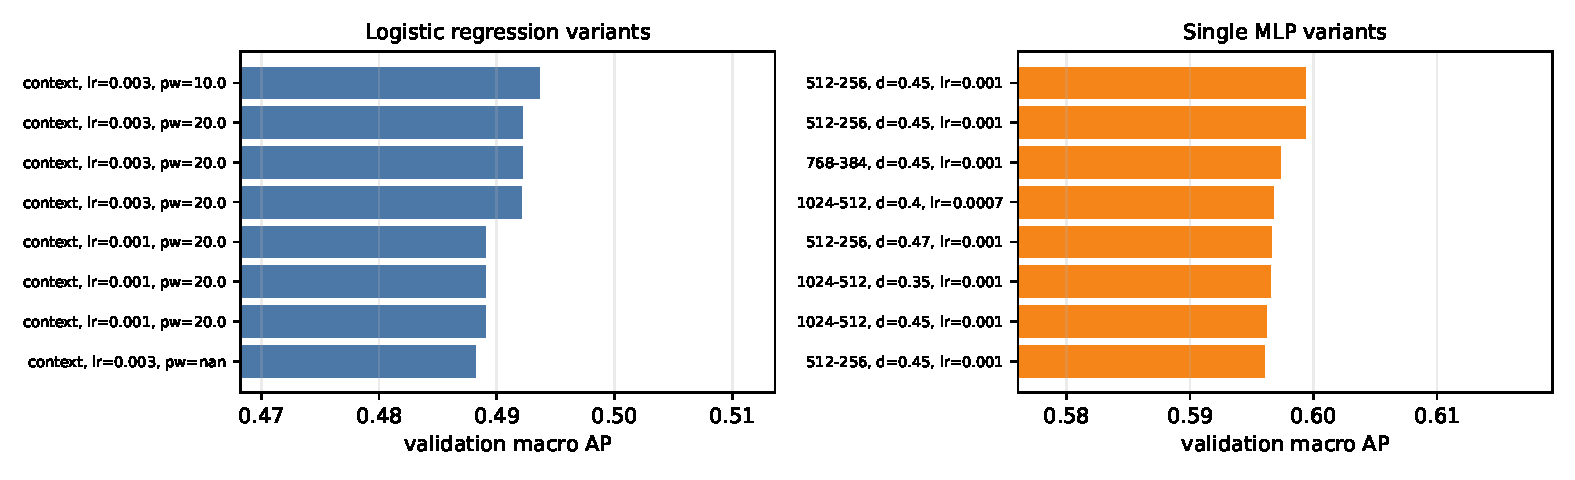
\includegraphics[width=0.98\linewidth]{figures/hyperparameter_summary.pdf}
    \end{column}
  \end{columns}
\end{frame}

%% Slide 2: Qualitative cases
\begin{frame}{Qualitative Case Studies}
  \begin{columns}[T]
    \begin{column}{0.39\textwidth}
      \textbf{Success: file 000727}
      \begin{itemize}
        \item Kitchen: microwave, water, dishes
        \item Static phone recording
        \item File-level F1: \textbf{0.978}
        \item Sustained events align with mel-spectrogram energy
      \end{itemize}
      \vspace{0.6em}
      \textbf{Failure: file 000892}
      \begin{itemize}
        \item Hallway: door, footsteps, light switch
        \item Mobile phone recording
        \item File-level F1: \textbf{0.000}
        \item Short transients shifted or confused
      \end{itemize}
    \end{column}
    \begin{column}{0.58\textwidth}
      \centering
      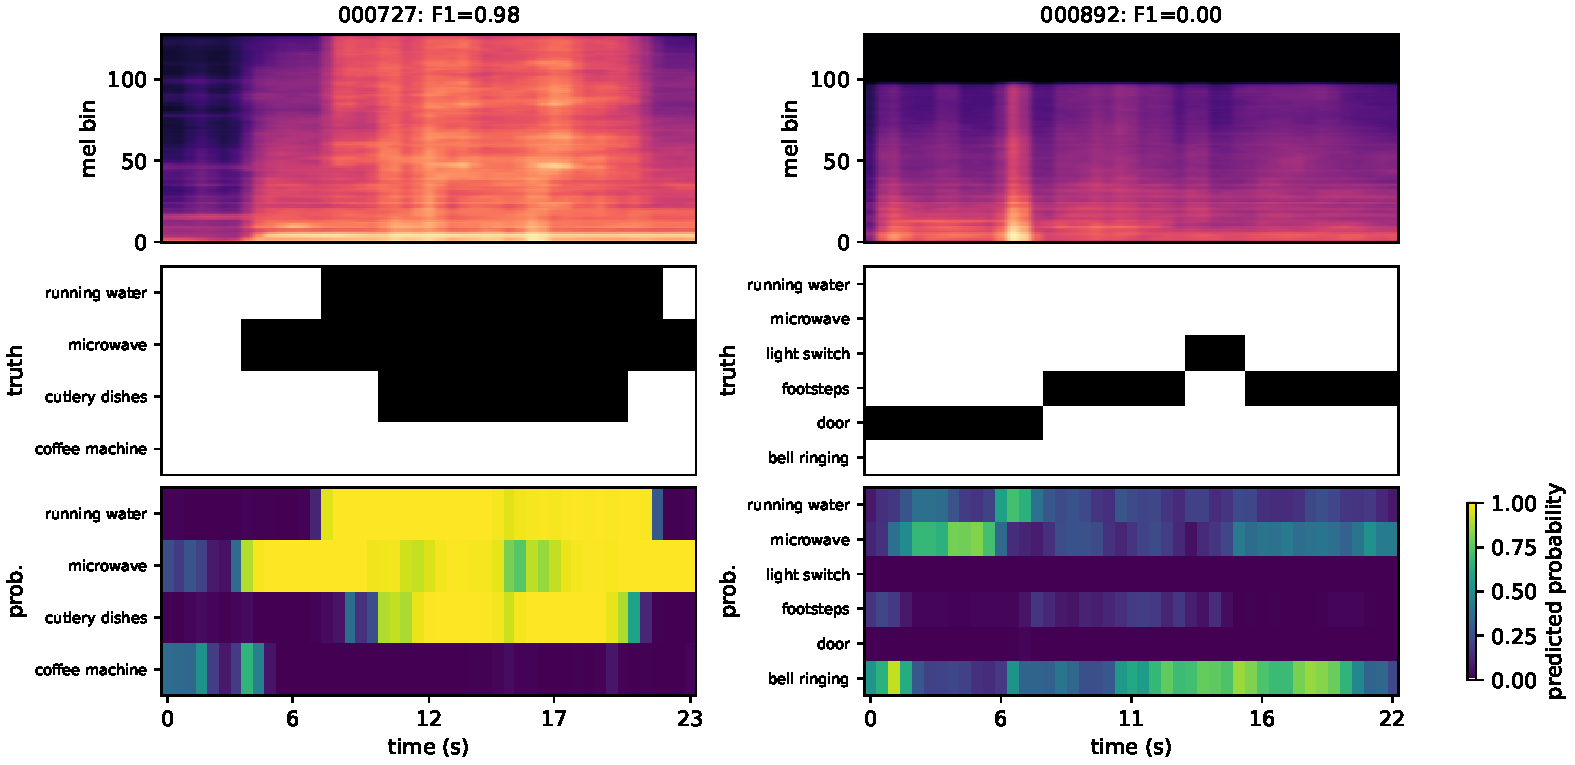
\includegraphics[width=\linewidth]{figures/case_studies.pdf}
    \end{column}
  \end{columns}
\end{frame}

%% Slide 3: Class-level strengths and weaknesses
\begin{frame}{What the Classifier Detects Reliably}
  \begin{columns}[T]
    \begin{column}{0.43\textwidth}
      \textbf{Reliable classes:}
      \begin{itemize}
        \item \texttt{running\_water}: 0.925 AP
        \item \texttt{keyboard\_typing}: 0.861 AP
        \item \texttt{vacuum\_cleaner}: 0.847 AP
        \item \texttt{microwave}: 0.793 AP
      \end{itemize}
      \vspace{0.6em}
      \textbf{Interpretation:}
      \begin{itemize}
        \item Sustained, repeated evidence across adjacent segments
        \item Distinct broadband or periodic spectral signatures
        \item Temporal context window helps stabilize predictions
      \end{itemize}
    \end{column}
    \begin{column}{0.55\textwidth}
      \centering
      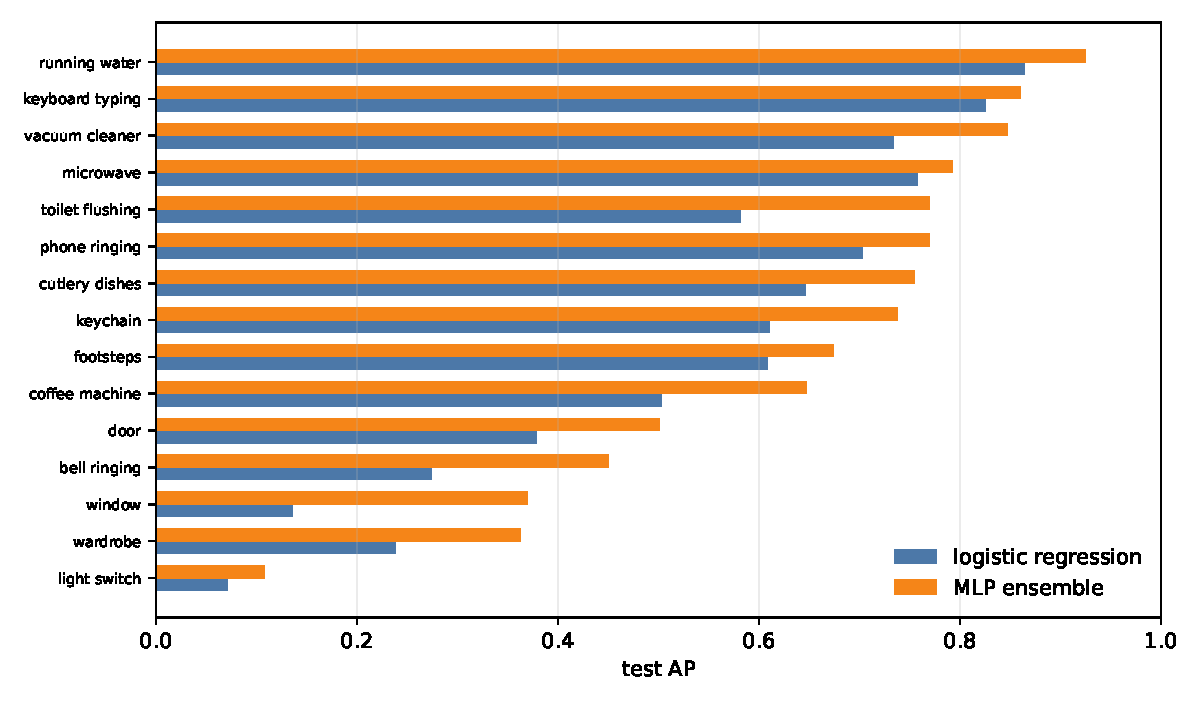
\includegraphics[width=\linewidth]{figures/per_class_ap.pdf}
    \end{column}
  \end{columns}
\end{frame}

%% Slide 4: Failure modes and next steps
\begin{frame}{Failure Modes and Next Steps}
  \begin{enumerate}
    \item \textbf{Short transients:}
    \texttt{light\_switch} remains hardest (0.108 AP); one-second aggregation and half-second hops can shift the evidence away from the label segment.

    \vspace{0.35em}
    \item \textbf{Mechanical confusions:}
    \texttt{door}, \texttt{window}, and \texttt{wardrobe\_drawer} share impact, hinge, and handling sounds; the feature representation separates them only weakly.

    \vspace{0.35em}
    \item \textbf{Rare-class instability:}
    Few positive examples make AP sensitive to label noise and missed annotator events.
  \end{enumerate}
  \vspace{0.6em}
  \textbf{Most promising improvements:}
  raw-audio temporal models, focal loss or rare-class sampling, explicit event-duration priors, and post-processing that smooths isolated false alarms without erasing real short events.
\end{frame}

\end{document}
